% 55 JAIIO - ASAID 2026
% Format: Springer LNCS, APA 7, anonymized submission
% Structure: EN title/abstract first, then ES, then body
%
\documentclass{llncs}

\usepackage[T1]{fontenc}
\usepackage{graphicx}
\usepackage{amsmath}
\usepackage{amssymb}
\usepackage{booktabs}
\usepackage{microtype}
\usepackage[htt]{hyphenat}
\emergencystretch=1.5em
\usepackage[style=apa]{biblatex}
\addbibresource{references.bib}

\begin{document}

% --- ENGLISH TITLE AND ABSTRACT (first, per 55 JAIIO 2026 rules) ---

\title{Not All Instructions Are Forgotten Equal}

% Anonymized for submission
\author{}
\institute{}

\maketitle

\begin{abstract}
Large language models lose adherence to user-stated preferences over
extended coding conversations, even when system prompt instructions
remain stable. We investigate this per-instruction retention
heterogeneity using a Bayesian ordered logistic model fitted to 244
compliance observations across 5 models, 12 decision types, and 3
real-world codebases. We find that treatment effects vary by over an
order of magnitude: some preferences are retained when stated,
others are ignored, and one is actively harmed by reinforcement. These
results establish the empirical prerequisite for selective reinforcement:
the per-instruction heterogeneity that a Bayesian Knowledge Tracing
system would need to exploit. A posterior-derived reinforcement ranking
identifies that 3 of 12 instruction types benefit from reinforcement,
1 should never be reinforced, and 8 require no intervention.

\keywords{instruction compliance \and context rot \and Bayesian inference
\and selective reinforcement \and LLM evaluation}
\end{abstract}

% --- SPANISH TITLE AND ABSTRACT ---

\begin{center}
\vspace{1cm}
{\Large \bfseries\boldmath No Todas las Instrucciones se Olvidan Igual}
\vspace{0.5cm}
\end{center}

\begin{abstract}
Los modelos de lenguaje grandes pierden adherencia a las preferencias
del usuario a lo largo de conversaciones extendidas de programaci\'on,
incluso cuando las instrucciones del system prompt se mantienen estables.
Investigamos esta heterogeneidad en la retenci\'on por tipo de
instrucci\'on usando un modelo log\'istico ordinal bayesiano ajustado a
244 observaciones de cumplimiento en 5 modelos, 12 tipos de decisi\'on
y 3 codebases reales. Encontramos que los efectos del tratamiento
var\'ian en m\'as de un orden de magnitud: algunas preferencias se
retienen al ser establecidas, otras se ignoran, y una
empeora activamente con el refuerzo. Estos resultados establecen el prerrequisito emp\'irico para el
refuerzo selectivo: la heterogeneidad por tipo de instrucci\'on que un
sistema basado en Bayesian Knowledge Tracing necesitar\'ia explotar.

\keywords{cumplimiento de instrucciones \and degradaci\'on de contexto
\and inferencia bayesiana \and refuerzo selectivo \and evaluaci\'on de LLMs}
\end{abstract}

\vspace{0.5cm}
\setcounter{page}{1}

%% ============================================================
\section{Introduction}
\label{sec:intro}
%% ============================================================

Large language models lose adherence to instructions over extended
conversations, a phenomenon we refer to as \emph{context rot}.
\textcite{laban2025} measured average compliance drops of 39\% across 15
models in multi-turn settings. The cause is
architectural: attention is not uniformly distributed across the context
window, and information in middle positions receives less weight than
information at the boundaries \parencite{liu2024}. System prompt
instructions sit at position zero, where causal attention gives them a
logarithmic compounding advantage \parencite{chowdhury2026}. User-stated preferences, introduced
mid-conversation, get no such benefit. They compete for attention
against all the context that accumulates after them.

This matters because every reinforcement token costs money, and weakened
safety guardrails accumulate without detection over long sessions
\parencite{mu2025}. The current fix is to repeat all instructions every
turn. This multiplies prompt cost and still fails to distinguish between
instructions the model has retained and those it has forgotten.

No prior work has measured this heterogeneity at the level of individual
instructions. Existing studies report mean compliance across instruction
sets \parencite{laban2025, he2024} or propose uniform mitigation
strategies such as periodic reminders \parencite{dongre2025}. But if
each instruction decays at a different rate, the mean hides the
structure that matters. An instruction that is already retained does not
need reinforcement. An instruction that is harmed by repetition should
not receive it. Without per-instruction estimates, any reinforcement
policy is flying blind.

Bayesian Knowledge Tracing \parencite{corbett1994} offers a framework
for exactly this kind of estimation. Originally developed in education,
BKT estimates the probability that a student has mastered a concept
based on a sequence of observed responses. The conceptual inversion we
propose is to treat the LLM as the student and its instructions as the
concepts. A BKT-based reinforcement system would only be useful if instruction
retention is in fact heterogeneous. We test this using a Bayesian ordered logistic model with
hierarchical effects per decision type, fitted to compliance scores
collected from realistic multi-turn coding conversations across three
open-source codebases.

We report three findings. First, retention heterogeneity across
instruction types is large, with treatment effects on the log-odds scale
ranging from $-2.4$ to $+5.4$ (group-level standard deviation
$\sigma_\beta = 2.1$). Second, one instruction type
(\texttt{dependencies\_no\_new}) is actively harmed by reinforcement,
with compliance dropping when the preference is stated. Third, we find little
evidence that model architecture or codebase size explains meaningful
variance in retention; the resolvable variation is almost entirely in the
instruction type itself. These results establish that selective reinforcement is necessary,
and that a Bayesian model can identify which
instructions to reinforce, which to leave alone, and which to never
mention again.


%% ============================================================
\section{Related work}
\label{sec:related}
%% ============================================================

\paragraph{Instruction compliance degradation.}
Several recent studies have established that LLMs lose adherence to
instructions as conversations grow. \textcite{laban2025} documented an
average 39\% compliance drop across 15 models in multi-turn settings
over 200K conversations. \textcite{he2024} showed that accuracy on
multi-instruction tasks drops from 87.7\% to 70.7\% within three turns,
even when instructions are given simultaneously. \textcite{du2025}
demonstrated that increasing the context window alone does not resolve
this degradation. All three studies report aggregate metrics across
instruction types. None examines whether different instructions degrade
at different rates.

\paragraph{Positional attention and prompt saturation.}
The mechanism behind compliance degradation has roots in the attention
architecture itself. \textcite{liu2024} identified a U-shaped attention
curve: information at the beginning and end of the context receives more
weight, while middle positions are underweighted. This positional bias
explains why system prompt instructions, which occupy position zero,
remain more stable than user-stated preferences buried mid-conversation.
\textcite{mu2025} showed a related saturation effect: as the number of
guardrails in a system prompt increases, compliance with any individual
rule drops sharply. Together, these results suggest that instruction adherence degrades
unevenly, shaped by where an instruction sits in the context and how
many others surround it.

\paragraph{Uniform mitigation strategies.}
Existing approaches to maintaining compliance treat all instructions
equally. \textcite{dongre2025} modeled instruction drift as a bounded
stochastic process and proposed periodic reminders to reduce divergence.
\textcite{leviathan2025} studied the effect of prompt repetition on
instruction stability. Both approaches reinforce all instructions at
each intervention, regardless of whether an individual instruction has
been retained or forgotten. This uniform strategy becomes expensive at
scale and, as our results show, can be counterproductive for
instructions where repetition degrades compliance.

\paragraph{Bayesian models of LLM behavior.}
\textcite{zhang2025} demonstrated that LLMs behave as discounted
Bayesian filters with a discount factor $\gamma < 1$, meaning that
prior beliefs are systematically downweighted relative to recent
observations. They measured this using controlled probabilistic probes
(biased dice, Gaussian mean estimation) where ground-truth parameters
shift and the model must adapt. Their work established that LLM
forgetting has Bayesian structure, but did not measure whether
$\gamma$ varies across instruction types. In education, Bayesian
Knowledge Tracing \parencite{corbett1994} has tracked per-concept
mastery probabilities for over 30 years. We apply this same logic in
reverse: rather than tracking what a student has learned, we track what
an LLM has forgotten, and we show that the per-instruction heterogeneity
that makes BKT useful in education also appears in LLM instruction
compliance.


%% ============================================================
\section{Method}
\label{sec:method}
%% ============================================================

\subsection{Decision planting protocol}
\label{sec:planting}

We simulate an AI coding assistant working on a real open-source
codebase over 25 turns. At each turn, the assistant receives a user
message and may call tools (read files, write code, search the
codebase). Real source files are injected into the conversation at
turns 0--19, building up context pressure as the conversation
progresses.

In the \textbf{treatment} condition, 12 coding preferences are embedded
as casual inline requests within the user's messages at specific turns.
Six are planted early (turns 1--7) and six late (turns 14--19). Each
preference targets a different coding practice: code style (numpy
broadcasting, list comprehensions), architecture (subclassing vs
standalone functions), testing (parametrize, approximate assertions),
naming (underscore prefix, no abbreviations), dependencies (no new
imports, module-level constants), and documentation (NumPy-style
docstrings, regex comments). The instructions are phrased as natural
user preferences, not system prompt rules (e.g., ``Important: when
writing array operations for this project, always use numpy
broadcasting instead of for loops'').

In the \textbf{baseline} condition, the conversation follows the same
structure with the same file injections and the same task, but no
preferences are planted. This allows us to measure what the model does
by default for each decision type.

At turns 20--25, the user requests code generation tasks designed to
elicit each decision. Each test turn evaluates exactly two decisions
(one early-planted, one late-planted), and the model's code output is
scored by deterministic checkers.

\subsection{Compliance measurement}
\label{sec:measurement}

Each of the 12 decision types is evaluated by a deterministic checker
that parses the model's code output using regular expressions and
pattern matching. Checkers are fully automated with no LLM-in-the-loop
evaluation. This makes results reproducible across runs. Each checker produces
an ordinal score on a 0--3 scale:

\begin{itemize}
  \item \textbf{0}: Completely ignored or violated
  \item \textbf{1}: Minimal or inconsistent compliance
  \item \textbf{2}: Mostly followed with minor deviations
  \item \textbf{3}: Fully followed
\end{itemize}

\begin{sloppypar}
For example, the \texttt{parametrize} checker searches for
\texttt{pytest.mark.parametrize} decorators and penalizes separate
test functions. The \texttt{broadcasting} checker detects
\texttt{for} loops and rewards numpy operations. The
\texttt{no\_new\_imports} checker counts \texttt{import} statements
in generated code.
\end{sloppypar}

\subsection{Bayesian model}
\label{sec:bayesian-model}

We model the ordinal compliance scores using an ordered logistic
regression (cumulative link model) with hierarchical effects per
decision type. The ordered logistic is appropriate because the 0--3
scores have unequal intervals: the gap between 0 (ignored) and 1
(minimal compliance) is qualitatively different from the gap between 2
(mostly followed) and 3 (fully followed). A linear model would
incorrectly assume equal spacing.

For each observation $i$, the latent compliance $\eta_i$ is:
\begin{equation}
  \eta_i = \alpha_{d[i]} + \beta_{d[i]} \cdot \text{treatment}_i
\end{equation}
where $d[i]$ indexes the decision type, $\alpha_d$ is the baseline
intercept (compliance without being told), and $\beta_d$ is the
treatment effect (how much telling improves compliance). The observed
score is determined by where $\eta$ falls relative to three ordered
cutpoints $c_1 < c_2 < c_3$.

Both $\alpha$ and $\beta$ are given hierarchical priors with
non-centered parameterization:
\begin{align}
  \alpha_d &= \mu_\alpha + \sigma_\alpha \cdot \tilde{\alpha}_d, \quad
    \tilde{\alpha}_d \sim \text{Normal}(0, 1) \\
  \beta_d &= \mu_\beta + \sigma_\beta \cdot \tilde{\beta}_d, \quad
    \tilde{\beta}_d \sim \text{Normal}(0, 1)
\end{align}

The hyperpriors are weakly informative on the log-odds scale:
$\mu_\alpha \sim \text{Normal}(0, 1.5)$,
$\mu_\beta \sim \text{Normal}(0, 1)$ (centered at zero, no prior
assumption about direction),
$\sigma_\alpha, \sigma_\beta \sim \text{Exp}(1)$.
Cutpoints use an offset parameterization:
$c_1 \sim \text{Normal}(0, 1.5)$ with positive increments
$\Delta c \sim \text{Exp}(1)$ to guarantee ordering.

The key scientific parameter is $\sigma_\beta$: the group-level
standard deviation of treatment effects. A large $\sigma_\beta$
indicates that different instructions respond differently to being
stated, which is the premise required for selective reinforcement.

We initially fit a full model including per-model and per-codebase
intercepts. Both had posterior group-level standard deviations near zero
($\sigma_\text{model} \approx 0.4$, $\sigma_\text{codebase} \approx
0.3$) with all individual effects having credible intervals crossing
zero, and the model produced 267 divergent transitions. We removed
these terms and confirmed via the simplified model's clean diagnostics
(zero divergences, all $\hat{R} \leq 1.01$, minimum ESS $= 1311$) that
the data does not support meaningful model or codebase effects.

The model was implemented in PyMC \parencite{pymc2023}. Posterior
samples were drawn using the No-U-Turn Sampler
\parencite[NUTS;][]{hoffman2014} via the nutpie sampler, a Rust-based
NUTS implementation \parencite{nutpie2024}, with 4 chains of 1000
draws each following 1000 tuning steps. Prior predictive checks confirmed that the priors
produce plausible score distributions before fitting. Posterior
predictive checks verified that the fitted model reproduces the observed
data.


%% ============================================================
\section{Experimental setup}
\label{sec:setup}
%% ============================================================

\subsection{Codebases}

We selected three open-source Python libraries from the Bayesian
statistics ecosystem, chosen to span a range of codebase sizes and
thus context pressure levels:

\begin{itemize}
  \item \textbf{Bambi} ($\sim$10K lines): a high-level interface for
    Bayesian regression. By turn~20, injected files produce
    approximately 98K tokens of context.
  \item \textbf{ArviZ} ($\sim$25K lines): a library for exploratory
    analysis of Bayesian models. Context reaches approximately 160K
    tokens by turn~20.
  \item \textbf{PyMC} ($\sim$57K lines): a probabilistic programming
    framework. Context reaches approximately 203K tokens by turn~20.
\end{itemize}

All repositories were cloned at fixed commits: Bambi
(\texttt{5110615}, 2026-03-17), ArviZ (\texttt{arviz-base} at
\texttt{374cd28} and \texttt{arviz-stats} at \texttt{8d6316a},
2026-03-26/29), and PyMC (\texttt{bca2b1e}, 2026-03-27, branch v6).
Source files were injected into the conversation at turns 0--19 via
the tool execution system, which serves real file contents from the
cloned repositories.

\subsection{Models}

We evaluated five instruction-following models across two experiment
phases. Table~\ref{tab:models} summarizes the models and conditions.

\begin{table}[t]
\caption{Models and experimental conditions. Only Qwen was tested in
both baseline and treatment conditions.}\label{tab:models}
\centering
\begin{tabular}{llcc}
\toprule
Model & Parameters & Baseline & Treatment \\
\midrule
Qwen 3.5        & 27B  & \checkmark & \checkmark \\
Gemini 3.1 Flash Lite & --   &            & \checkmark \\
GPT-5.4-nano    & --   &            & \checkmark \\
Nemotron 3 Super & 120B &            & \checkmark \\
Gemma 4         & 26B  &            & \checkmark \\
\bottomrule
\end{tabular}
\end{table}

Qwen served as the primary model with both baseline and treatment
conditions across all three codebases (18 conversations). The remaining
four models were tested in the treatment condition only, to verify that
the retention patterns generalize across architectures. Gemma was tested
on Bambi only due to budget constraints.

\subsection{Dataset}

We ran 28 conversations in total: 9 baseline and 19 treatment. Models
were accessed through OpenRouter (Qwen, Gemini, Gemma, Nemotron) and
the OpenAI API (GPT-5.4-nano). Not every conversation produced a
scorable response at every test turn; the final dataset consists of 244
compliance observations: each observation is one decision type scored
at one test turn in one conversation. Observations span 5 models, 12
decision types, 3 codebases, and 2 conditions. The baseline condition
contributes 70 observations (all from Qwen), and the treatment
condition contributes 174 observations across all five models. All
conversation logs, checker code, and analysis notebooks are available
in the supplementary material.


%% ============================================================
\section{Results}
\label{sec:results}
%% ============================================================

The model converged cleanly: zero divergences, $\hat{R} \leq 1.01$
for all parameters, and a minimum effective sample size of 1311.
Posterior predictive checks confirm that the model reproduces the
observed score distribution (Figure~\ref{fig:ppc}).

\begin{figure}[t]
\centering
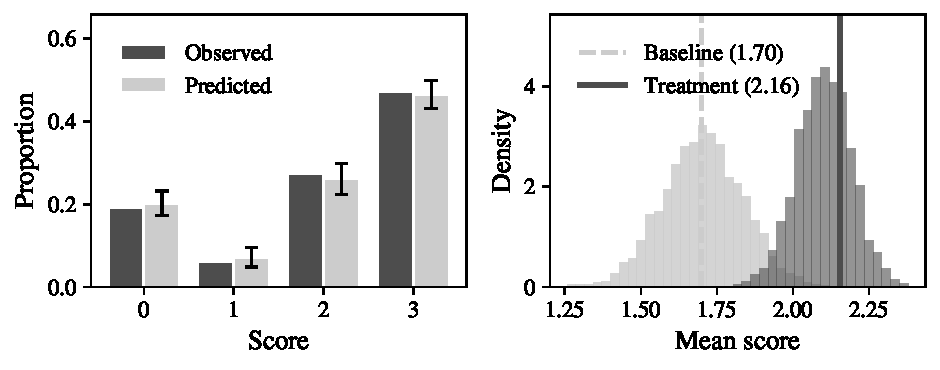
\includegraphics[width=\textwidth]{figures/posterior_predictive_check.pdf}
\caption{Posterior predictive check. Left: the model reproduces the
observed score distribution across all four ordinal categories. Right:
the model captures the difference in mean compliance between baseline
(1.70) and treatment (2.16) conditions.}\label{fig:ppc}
\end{figure}

\subsection{Treatment effect heterogeneity}

The group-level standard deviation of treatment effects is
$\sigma_\beta = 2.11$ (94\% HDI: $[1.06, 3.28]$), indicating that
different instruction types respond differently to being stated.
Individual treatment effects on the log-odds scale range from $-2.36$
to $+5.44$ (Figure~\ref{fig:forest}).

\begin{figure}[t]
\centering
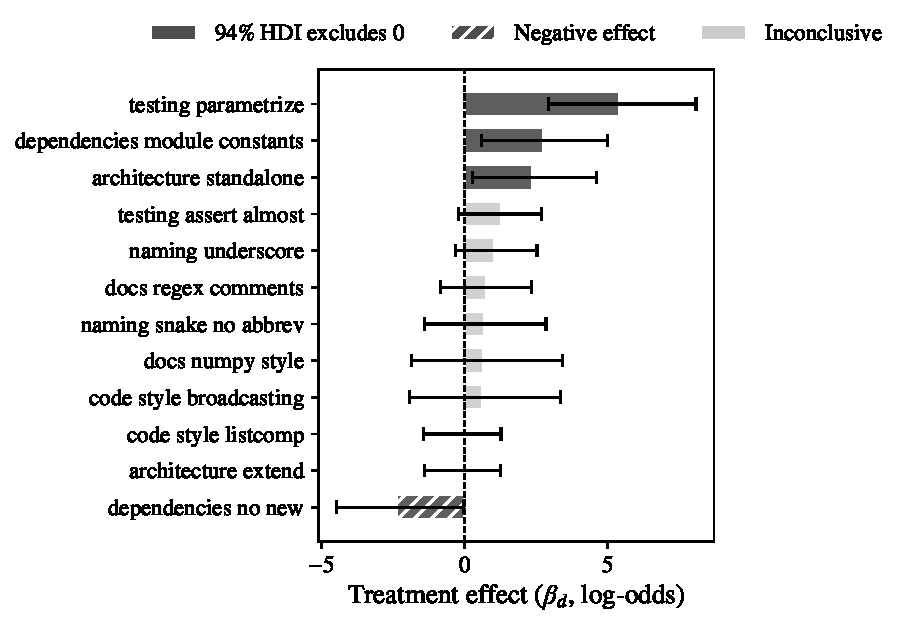
\includegraphics[width=0.85\textwidth]{figures/treatment_effects_forest.pdf}
\caption{Per-decision treatment effects ($\beta_d$) with 94\% HDI.
Dark bars: 94\% HDI excludes zero. Hatched: negative effect.
Light bars: inconclusive.}\label{fig:forest}
\end{figure}

The posterior separates the 12 decision types into three groups:

\paragraph{Instructions that benefit from reinforcement.}
Three decision types have treatment effects with 94\% HDI entirely
above zero. \texttt{testing\_parametrize} has the largest effect
($\beta = 5.44$, HDI: $[2.94, 8.10]$): models almost never use
\texttt{pytest.mark.\allowbreak{}parametrize} unprompted (baseline
mean: 0.00) but retain the preference when told (treatment mean:
2.79). \texttt{dependencies\_\allowbreak{}module\_constants}
($\beta = 2.76$, HDI: $[0.60, 5.00]$) and
\texttt{architecture\_\allowbreak{}standalone} ($\beta = 2.38$,
HDI: $[0.29, 4.63]$) follow the same pattern: near-zero baseline,
meaningful retention when stated.

\paragraph{An instruction harmed by reinforcement.}
\texttt{dependencies\_no\_new} ($\beta = -2.36$, HDI:
$[-4.46, -0.03]$) is the only decision type where telling the model
reduces compliance. The baseline mean score is 2.25 (models naturally
avoid adding imports), but stating ``do not add new imports'' drops the
treatment mean to 0.77. We hypothesize that the explicit negation
confuses the model's instruction following. Testing this would require
isolating the negation from the instruction content, e.g., comparing
``avoid new imports'' with ``use only existing imports.''

\paragraph{Instructions that need no intervention.}
The remaining eight decision types show treatment effects with HDIs
crossing zero. Several of these have high baseline compliance
(\texttt{broadcasting}: 3.00, \texttt{numpy\_style}: 3.00,
\texttt{snake\_no\_abbrev}: 2.67), meaning models already follow these
conventions without prompting. Reinforcing these would waste tokens.

\subsection{Model and codebase effects}

As described in Section~\ref{sec:bayesian-model}, we initially fit a
model with per-model and per-codebase intercepts. Both had posterior
group-level standard deviations near zero ($\sigma_\text{model} \approx
0.4$, $\sigma_\text{codebase} \approx 0.3$) and produced 267
divergences. The simplified model without these terms fits cleanly.

The retention landscape is consistent across
five model architectures (ranging from 26B to 120B parameters) and
three levels of context pressure (98K to 203K tokens). Within the
resolution of this design, what determines whether an instruction is
retained is the instruction itself rather than the model processing it or
the amount of surrounding context; we caution that the baseline condition
comes from a single model (Section~\ref{sec:discussion}), so per-model
retention cannot be fully separated.

\subsection{Reinforcement priorities}

We use the posterior to derive a reinforcement ranking. For each
decision type $d$, we compute $P(\text{score} \geq 2 \mid
\text{told})$ and $P(\text{score} \geq 2 \mid \text{not told})$ across
all posterior samples, and define the reinforcement gain as their
difference (Figure~\ref{fig:policy}). This is not a closed-loop policy
evaluation; it is a posterior-derived priority ranking that identifies
which instructions would benefit from reinforcement.

\begin{figure}[t]
\centering
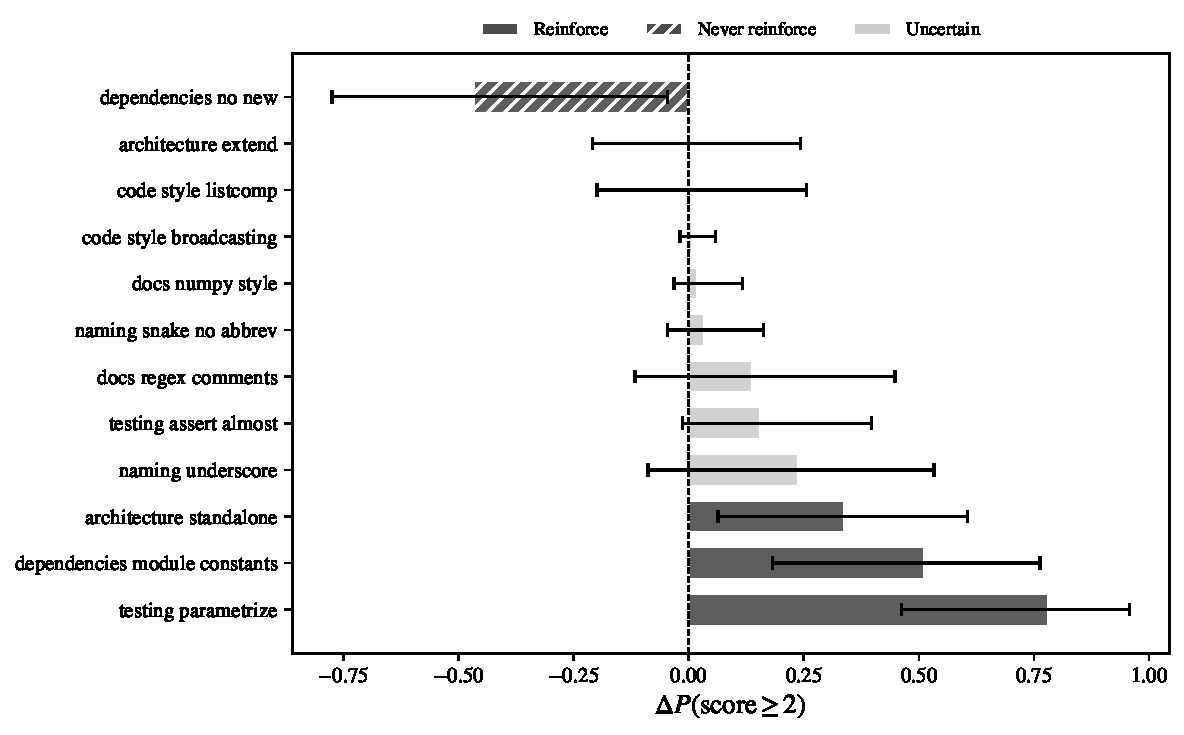
\includegraphics[width=\textwidth]{figures/reinforcement_policy.pdf}
\caption{Expected change in $P(\text{score} \geq 2)$ from reinforcing
each decision, with 94\% HDI. Dark bars: HDI excludes zero.
Hatched: reinforcement is harmful.}\label{fig:policy}
\end{figure}

Table~\ref{tab:policy} summarizes the ranking. Of 12 instruction types,
only 3 have a reinforcement gain with 94\% HDI entirely above zero. A
uniform policy that reinforces all 12 would spend tokens on 8
instructions that need no help and 1 that is actively harmed by
repetition.

\begin{table}[t]
\caption{Reinforcement priorities derived from posterior
estimates. Gain is $\Delta P(\text{score} \geq 2)$ from
reinforcement.}\label{tab:policy}
\centering
\begin{tabular}{lrrl}
\toprule
Decision type & Gain & 94\% HDI & Action \\
\midrule
\texttt{testing\_parametrize}    & $+$0.78 & $[+0.46, +0.96]$ & Reinforce \\
\texttt{module\_constants}       & $+$0.51 & $[+0.18, +0.76]$ & Reinforce \\
\texttt{arch\_standalone}        & $+$0.34 & $[+0.06, +0.61]$ & Reinforce \\
\texttt{naming\_underscore}      & $+$0.24 & $[-0.09, +0.53]$ & Uncertain \\
\texttt{testing\_assert\_almost} & $+$0.16 & $[-0.01, +0.40]$ & Uncertain \\
\texttt{docs\_regex\_comments}   & $+$0.14 & $[-0.12, +0.45]$ & Uncertain \\
\texttt{5 other types}           & $< +0.04$ & crosses zero & Skip \\
\texttt{deps\_no\_new}           & $-$0.47 & $[-0.77, -0.05]$ & Never reinforce \\
\bottomrule
\end{tabular}
\end{table}


%% ============================================================
\section{Discussion}
\label{sec:discussion}
%% ============================================================

\subsection{What determines retention}

The treatment effects follow a pattern: instructions that ask for
something the model would not do by default are retained when stated,
while instructions that match existing behavior show no treatment
effect. The three decisions with clear positive effects
(\texttt{parametrize}, \texttt{module\_constants},
\texttt{standalone}) all have baseline compliance near zero. The
decisions with no treatment effect (\texttt{broadcasting},
\texttt{numpy\_style}, \texttt{snake\_no\_abbrev}) have baseline
compliance near 3.0. The models' defaults already match these
conventions, so restating them buys nothing.

The negative effect on \texttt{dependencies\_\allowbreak{}no\_new}
($P(\beta < 0) = 0.98$) deserves separate attention. The instruction
``do not add new imports'' is the only one phrased as a negation. All
other instructions tell the model what to do, not what to avoid. This
raises the question of whether the negative treatment effect reflects
something about the content of the instruction (import management) or
its framing (negation). The answer matters for practitioners: if
negation is the problem, reformulating as ``use only existing imports''
might recover the positive effect. If import management is inherently
hard to retain, no framing will help. Distinguishing these hypotheses
requires a controlled comparison that holds semantic content constant
while varying the negation frame. As a reviewer noted, the sharpest
version of this test re-runs the instructions whose treatment effect
excludes zero under negated paraphrases, and the negated instruction
under positive paraphrases, so that within-instruction phrasing variance
can be measured against between-instruction variance; we adopt this
design in the future work below.

\subsection{Robustness checks}

To address the concern that baseline data comes from Qwen only, we
fit the same model restricted to Qwen observations (132 of 244,
both conditions). The per-decision treatment effects correlate at
$r = 0.80$ with the full-model estimates, and the group-level
heterogeneity parameter remains stable ($\sigma_\beta = 2.35$ vs.\
$2.11$ in the full model). The three strongest effects replicate:
\texttt{parametrize} ($\beta = 6.13$), \texttt{module\_constants}
($\beta = 2.25$), and \texttt{dependencies\_no\_new} ($\beta =
-1.07$, still negative though with wider intervals).

One decision, \texttt{architecture\_standalone}, does not replicate in
the Qwen-only analysis ($\beta = 2.38$ in the full model vs.\
$\beta = -0.71$ with Qwen alone). Its treatment effect in the full
model appears driven by the other four models. We reduce the count of
clearly beneficial decisions from three to two when considering only
Qwen data.

Leave-one-out cross-validation shows no problematic observations
(all Pareto $\hat{k} < 0.7$, ELPD = $-228.8 \pm 14.5$). Per-decision
posterior predictive checks confirm that the model reproduces the
observed mean score for all 12 decision types within the 90\%
predictive interval (Figure~\ref{fig:ppc_decision}).

\begin{figure}[t]
\centering
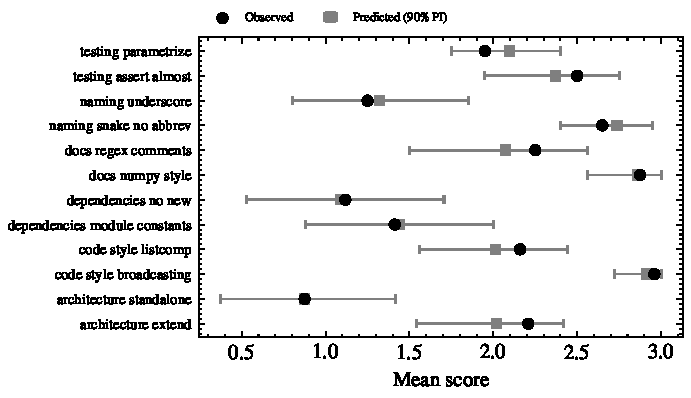
\includegraphics[width=\textwidth]{figures/ppc_per_decision.pdf}
\caption{Per-decision posterior predictive check. Observed means
(dots) fall within the 90\% posterior predictive interval for all 12
decision types.}\label{fig:ppc_decision}
\end{figure}

\subsection{Limitations}

Baseline data comes from one model only (Qwen). The sensitivity
analysis ($r = 0.80$) mitigates but does not eliminate this concern.
Future replications should include baseline conditions for every model
tested.

The dataset contains 244 observations, with some decision-by-condition
cells containing as few as 4 observations. The hierarchical model
handles sparsity through partial pooling, and the wide credible
intervals for low-data decisions reflect this uncertainty honestly.
However, the reinforcement ranking for the ``uncertain'' category
(Table~\ref{tab:policy}) should be treated as preliminary.

Compliance was measured at turns 20--25 only. This gives a retention
snapshot, not a decay curve. We cannot estimate per-instruction decay
rates ($\gamma$ in the BKT framework) or determine at which turn
compliance begins to drop. Fitting actual forgetting curves would
require compliance measurements at every turn, which in turn requires
designing prompts that give the model an opportunity to demonstrate
each decision at each turn without making the conversation artificial.

The deterministic checkers have construct validity limitations. When a
checker cannot find a relevant code pattern, it defaults to a score of
2 (``no clear signal''). Four decision types have default-2 rates
above 50\%: \texttt{architecture\_extend} (79\%),
\texttt{docs\_regex\_comments} (75\%), \texttt{code\_style\_listcomp}
(72\%), and \texttt{testing\_assert\_almost} (50\%). The three
decisions with the strongest treatment effects (\texttt{parametrize},
\texttt{standalone}, \texttt{no\_new}) have 0\% default-2 rates, so
the headline findings are not driven by this artifact. The
\texttt{no\_new\_imports} checker penalizes any \texttt{import}
statement, including standard library modules that may be required by
the task.

This paper does not implement Bayesian Knowledge Tracing. It measures
the per-instruction heterogeneity that would make a BKT-based
reinforcement system useful. Building and evaluating such a system,
including closed-loop token-budget allocation and real-time compliance
tracking, is future work.

\subsection{Future work}

Six directions follow from these results and from reviewer feedback.

\emph{Full-factorial baselines and broader model coverage.} Our baseline
condition was collected for a single model (Qwen); extending matched
baseline and treatment conditions to every model would let us estimate
per-model effects directly and test whether the retention landscape is
model-invariant, rather than inferring it from a single-model sensitivity
analysis.

\emph{Triangulated, debiased compliance measurement.} The deterministic
checkers are fully reproducible but have construct-validity limits (high
default-score rates for some decisions). Pairing them with a blinded
panel of LLM judges drawn from model families distinct from those under
evaluation, and reporting checker--judge and inter-judge agreement, would
separate measurement bias from the effect of interest.

\emph{Disentangling phrasing from instruction type.} The only instruction
harmed by reinforcement (\texttt{dependencies\_no\_new}) is also the only
one phrased as a negation. Re-running the instructions whose treatment
effect excludes zero under negated paraphrases, and the negated
instruction under positive paraphrases, would measure within-instruction
phrasing variance against between-instruction variance, isolating whether
negation framing rather than content drives the effect.

\emph{Dense temporal measurement.} Scoring compliance at every turn,
rather than only at turns 20--25, would let us fit per-instruction
forgetting curves and estimate decay rates (the discount factor in the
BKT framework).

\emph{Closed-loop evaluation.} Implementing the posterior-derived
reinforcement ranking as a runtime policy and measuring whether selective
reinforcement beats uniform reinforcement under a fixed token budget.

\emph{Ecological validity.} Replacing simulated planting with traces from
real coding sessions would test whether the retention structure observed
here holds outside the harness.

%% ============================================================
\section{Conclusion}
\label{sec:conclusion}
%% ============================================================

We measured per-instruction retention in AI coding assistants and found
that it varies by over an order of magnitude. Some instructions are
retained when stated, some are already followed by default, and one is
actively harmed by reinforcement. This heterogeneity is consistent
across five model architectures and three levels of context pressure,
and it replicates when the analysis is restricted to a single model
with matched baseline and treatment conditions ($r = 0.80$).

The practical implication is that uniform reinforcement strategies
waste most of their token budget. A posterior-derived ranking can
identify which instructions to reinforce and which to leave alone.
The per-instruction retention probabilities estimated here are the
input that a Bayesian Knowledge Tracing system would need to operate.
Building that system is the next step.


\begin{credits}
\subsubsection{\discintname}
The authors have no competing interests to declare that are relevant
to the content of this article.
\end{credits}

\printbibliography

\end{document}
